The purpose of the floor plan in the application is to be used as a navigation guide for the user. The user should be able to make a customised route to different booths, The default route should be a route between all the booths that the user has subscribed to.
Ideally it should also be possible to subscribe/unsubscribe to each booth. The location of the user is detected when the user scans an \ac{nfc} tag, the \ac{nfc} tag are placed around the exhibition and at booths, to provide the user with easy location determination.

\section{MapView vs MapFragment}
Our initial thought on how to implement the floor plan on the phone was to use the service provided by Google Maps. We knew that it could implemented on the phone because we had previously seen it being used in other applications. What we did not know, was if we could override the standard Google Maps tiles with our own custom tile set of the floor plan. A tile is a single picture containing a piece of the map, depending on the zoom level each tile contain a smaller piece of the actual map.\\
\todo{show what a tile looks like, side by side with Google Maps tile}
We need to implement our own custom tile set because we want to show the floor plan of a building, instead of a map of the Earth. We read the documentation provided by Google Maps\todo{cite?}, and we found that it is not possible to override the standard tiles with your own tiles to the Android MapFragment. We then thought of implementing the floor plan with a WebView which is basically a browser inside the application, and use JavaScript to create the map. With JavaScript it is possible to override the standard tile set with your own, but the performance on the phone was horrible so we scratched the idea. After some research we found a solution to our problem, we use a MapFragment and instead overriding the standard tile set we simply hide them, and only show our custom tile set of the floor plan.

\section{Mercator projection}
\label{sec:mercatorprojection}
\todo{introduction, why it is good to know(mercator projection)? because Google maps!!}
Mercator projection is a way of displaying a sphere on a two dimensional map.
There are a lot of ways of projecting a sphere on a map, but one of the most successful is the Mercator projection. The Mercator projection is often chosen because of it navigational properties strengths. One of the biggest navigational properties Mercator provides is it's ability to represent lines of constant course as straight lines.\\
A Mercator projected map is illustrated by Figure  \autoref{fig:mercatorexplain}. Let the globe be a spherical balloon, the balloon is blown up inside a cylinder, and sticks to the cylinders side as it is blown up. The three first pictures on Figure \autoref{fig:mercatorexplain} shows the balloon being blowing up, the last picture shows the cylinder being cut open and displayed as a two dimensional map.
\begin{figure}[H]
\centering
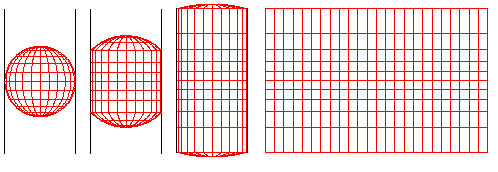
\includegraphics[width=0.8\textwidth]{img/mercatorexplain.png}
\caption{Explanation of Mercator projection \citep{mercatorexplain}}
\label{fig:mercatorexplain}
\end{figure}
The \autoref{fig:mercatorexplain} also shows how the top part of the spherical balloon is stretched for it to fit inside the cylinder. This is one of the disadvantages of the Mercator projection, the landmasses and continents are not scaled correctly.
\begin{figure}[H]
\centering
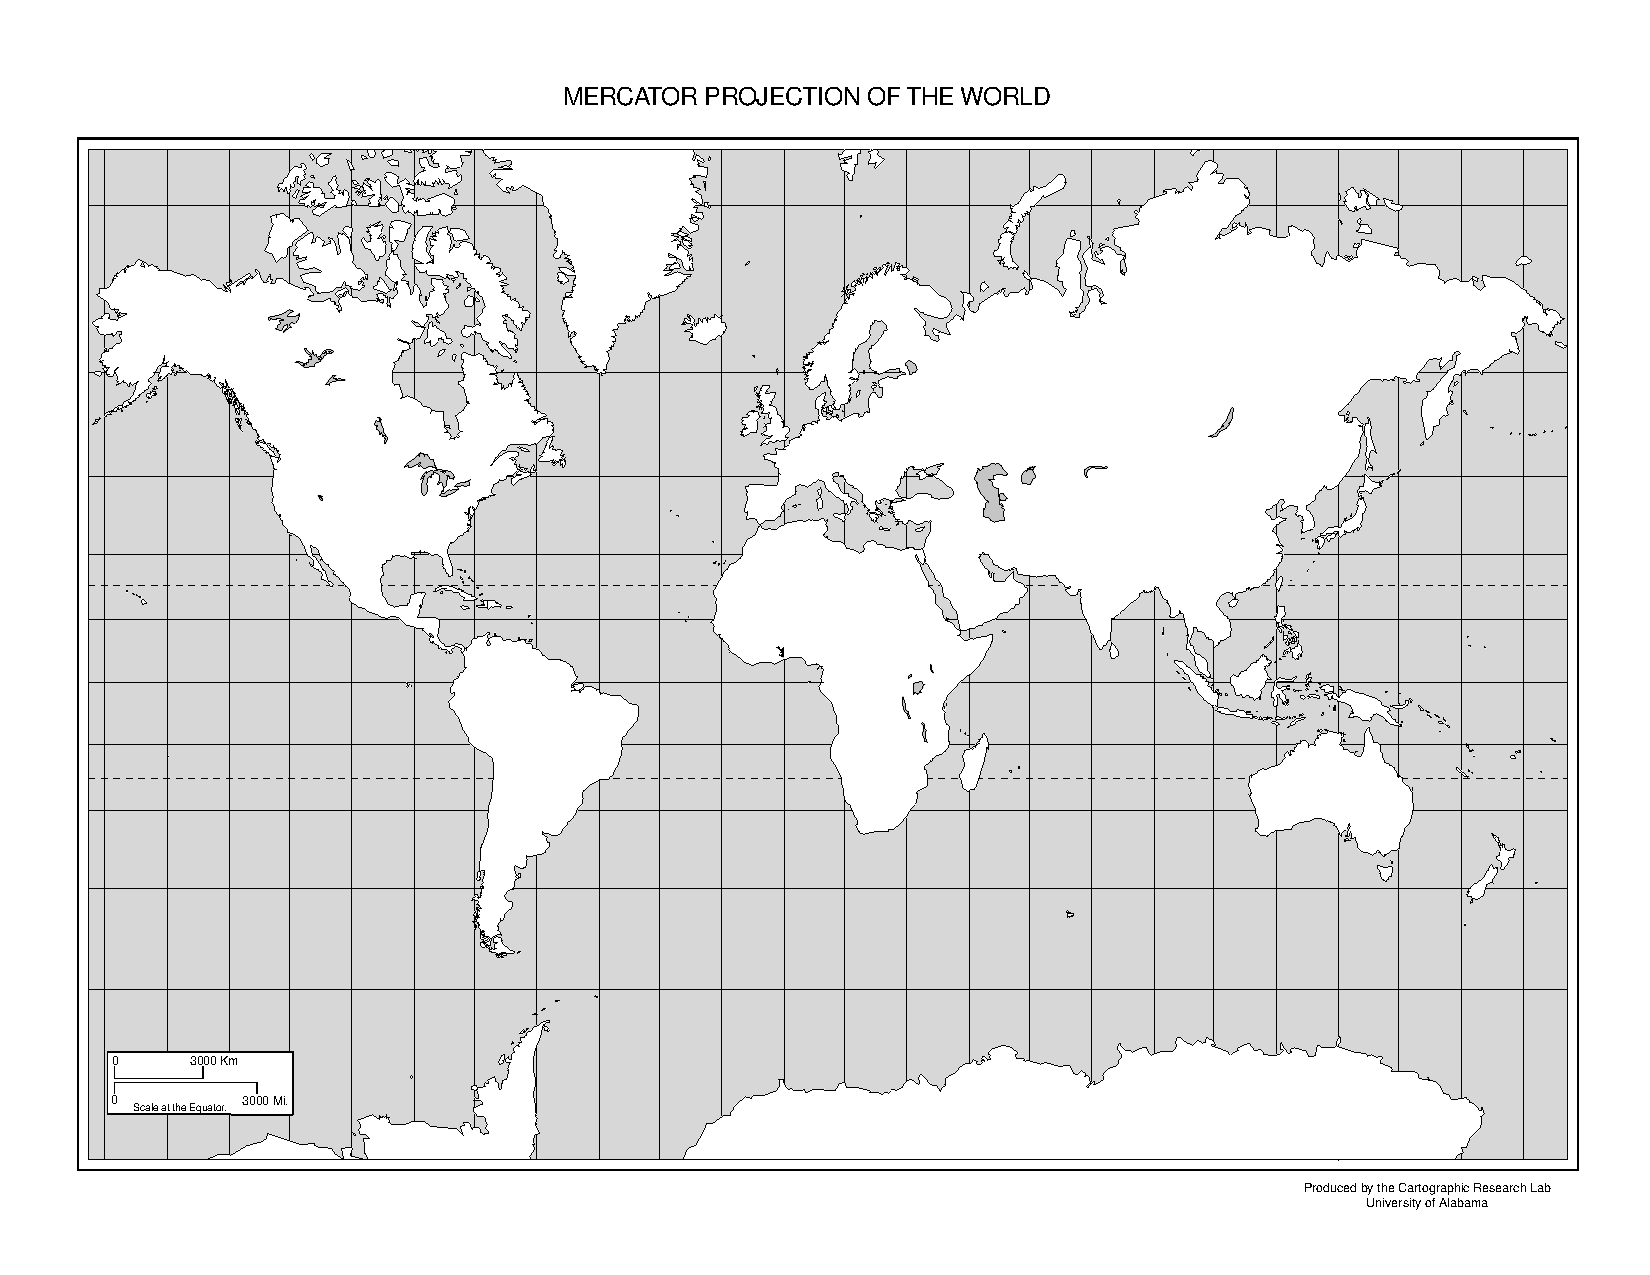
\includegraphics[width=0.8\textwidth]{img/mercatorworld.pdf}
\caption{The World - Mercator projection  \citep{mercatorworld}}
\label{fig:mercatorworld}
\end{figure} 
On the \autoref{fig:mercatorworld} Greenland is almost the same size as Africa, but in reality Africa is 14 times bigger than Greenland.

\section{Google Maps}
\todo{Explain the Google Maps \ac{api} for android} We use the service provided by Google, called Google Maps, to present our floor plan. This service is normally used for displaying the Earth and for navigation. Google Maps for projection of the Earth. Google Maps uses the Mercator projection which is explained in a earlier \secref{sec:mercatorprojection}. Normally a map is distorted by the Mercator projection, but in our case this is not a problem, since our floor plan already is a plane. 
\subsection*{Tiles}
The Google Maps \ac{api} allows the user to zoom on the floor plan, the floor plan is shown on \autoref{fig:floorplan}. Zooming on the floor plan allows us to present the floor plan in more detail. For this to work we need to split our original floor plan picture into small tiles, the tiles are always the size 256$x$256 pixels. As the zoom level increases the more tiles are needed to present the floor plan, so at zoom level 2 the floor plan will be rendered as  a 4$x$4 grid. At zoom level 3 a 8$x$8 grid, and so on. \autoref{fig:tilecoordinates} shows how the original picture is split into tiles on zoom level 2.

\begin{figure}[H]
\centering
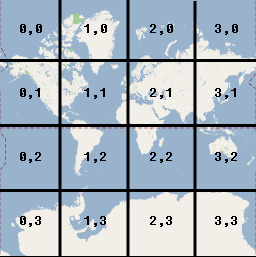
\includegraphics[width=0.5\textwidth]{img/tilecoordinates.png}
\caption{Tile split example with zoom level 2 \citep{tilecoordinates}}
\label{fig:tilecoordinates}
\end{figure}

\subsection*{Map Elements}
The Google Maps \ac{api} also allows us to draw different shapes and elements onto the floor plan. In this section we will show and explain how these elements are created and used.
\subsubsection*{Markers}

Markers how to make them? how they are structured, show examples
\subsubsection*{Polylines}

Polylines how to make them? how they are structured, show examples
\subsubsection*{Polygons}

Polygons how to make them? how they are structured, show examples
Long \& Latitude?\\


\section*{Implementation of Floor Plan} 
Explain how the tiles is loaded into the app(google map)\\
Explain how thing are loaded from the database.\\
Location stuff
	
